\documentclass[convert={density=300,size=600x400,outext=.png},crop,tikz]{standalone}% 'crop' is the default for v1.0, before it was 'preview'

% (Judit) This doesn't work:
%\usetikzlibrary{external}
%\tikzexternalize[mode=list and make]
%\dimendef\prevdepth=0

%\tikzset{
%    png export/.style={
%        % First we call ImageMagick; change settings to requirements
%        external/system call/.add={}{; convert -density 300 -transparent white "\image.pdf" "\image.png"},
%        % Now we force the PNG figure to be used instead of the PDF
%        /pgf/images/external info,
%        /pgf/images/include external/.code={
%            \includegraphics[width=\pgfexternalwidth,height=\pgfexternalheight]{##1.png}
%        },
%    }
%}
%\tikzset{png export}
\newcommand{\pad}{PAD}

\usepackage{xcolor}

\makeatletter
\newcommand{\gettikzxy}[3]{%
    \tikz@scan@one@point\pgfutil@firstofone#1\relax
    \edef#2{\the\pgf@x}%
    \edef#3{\the\pgf@y}%
}
\makeatother

% Tab10 color palette
\definecolor{tab1}{RGB}{30,118,179}
\definecolor{tab2}{RGB}{255,126,13}
\definecolor{tab3}{RGB}{43,159,43}
\definecolor{tab4}{RGB}{213,38,39}
\definecolor{tab5}{RGB}{147,102,188}
\definecolor{tab6}{RGB}{139,85,74}
\definecolor{tab7}{RGB}{226,118,193}
\definecolor{tab8}{RGB}{126,126,126}
\definecolor{tab9}{RGB}{187,188,33}
\definecolor{tab10}{RGB}{22,189,206}

\usepackage{tikz}
\usetikzlibrary{matrix,positioning,shapes.geometric, arrows, fit, decorations.pathreplacing}
\usetikzlibrary{calc}

\tikzstyle{box} = [
    rectangle, text centered,
    minimum width=.4cm,
    minimum height=1cm,
    thick,
]
\tikzstyle{input} = [
    box,
    fill=tab1!30,
    draw=tab1,
]
\tikzstyle{lastsymbol} = [
    fill=tab2!40,
]
\tikzstyle{pad} = [
    fill=tab8!20,
]
\tikzstyle{token} = [
    minimum width=1cm,
    minimum height=0.8cm,
]
\tikzstyle{dense} = [
    box,
    minimum width = 1cm,
    minimum height=0.8cm,
    fill=tab5!30,
    draw=tab5,
]
\tikzstyle{embedding} = [
    box,
    minimum width=7.5cm,
    minimum height=0.8cm,
    fill=tab8!30,
    draw=tab8,
]
\tikzstyle{hidden} = [
    box,
    fill=tab2!30,
    draw=tab2,
]
\tikzstyle{lstm} = [
    hidden,
    minimum height=0.8cm,
]
\tikzstyle{output} = [
    box,
    fill=tab3!30,
    draw=tab3,
]

\tikzstyle{arrow} = [->,>=stealth]
\tikzset{
    *|/.style={
        to path={
            (
            perpendicular cs: 
            horizontal line through={(\tikztostart)},
            vertical line through={(\tikztotarget)}
            )
            % is the same as (\tikztostart -| \tikztotarget)
            % but just to be safe: http://tex.stackexchange.com/a/29781/16595
            -- (\tikztotarget) \tikztonodes
        }
    }
}
%%%%%%%%%%%%%%%%%% END TIKZ %%%%%%%%%%%%%%%%%%%%

\begin{document}
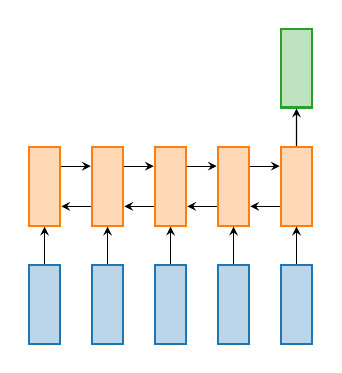
\begin{tikzpicture}
    % boxes
    \foreach \x in {1,...,5} {
        \node (in\x) at (0.8*\x, 0) [input] {};
        \node (hidden\x) at (0.8*\x, 1.5) [hidden] {};
    }

    \node (out) at (4, 3) [output] {};

    % arrows
    \foreach \x in {1,...,5}
        \draw [arrow] (in\x.north) to (hidden\x.south);

    \foreach \x [evaluate=\x as \y using int(\x+1)]  in {1,...,4} {
        \draw [arrow] (hidden\x.50) to (hidden\y.130);
        \draw [arrow] (hidden\y.230) to (hidden\x.310);
    }
    \draw [arrow] (hidden5.north) to (out.south);

\end{tikzpicture}
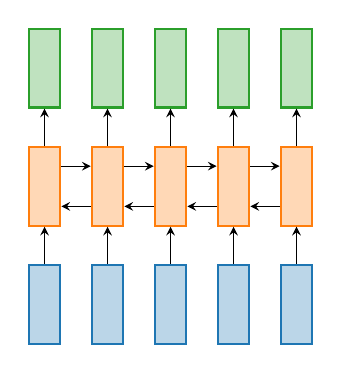
\begin{tikzpicture}
    % boxes
    \foreach \x in {1,...,5} {
        \node (in\x) at (0.8*\x, 0) [input] {};
        \node (hidden\x) at (0.8*\x, 1.5) [hidden] {};
        \node (out\x) at (0.8*\x, 3) [output] {};
    }

    % arrows
    \foreach \x in {1,...,5} {
        \draw [arrow] (in\x.north) to (hidden\x.south);
        \draw [arrow] (hidden\x.north) to (out\x.south);
    }

    \foreach \x [evaluate=\x as \y using int(\x+1)]  in {1,...,4} {
        \draw [arrow] (hidden\x.50) to (hidden\y.130);
        \draw [arrow] (hidden\y.230) to (hidden\x.310);
    }
\end{tikzpicture}
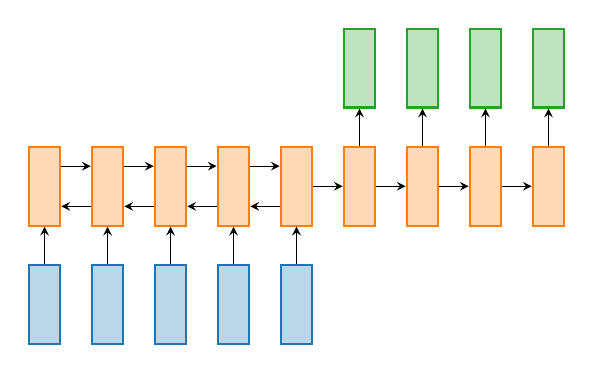
\begin{tikzpicture}
    % boxes
    \foreach \x in {1,...,5} {
        \node (in\x) at (0.8*\x, 0) [input] {};
        \node (hidden\x) at (0.8*\x, 1.5) [hidden] {};
    }
    \foreach \x in {6,...,9} {
        \node (hidden\x) at (0.8*\x, 1.5) [hidden] {};
        \node (out\x) at (0.8*\x, 3) [output] {};
    }

    % arrows
    \foreach \x in {1,...,5} {
        \draw [arrow] (in\x.north) to (hidden\x.south);
    }
    \foreach \x in {6,...,9} {
        \draw [arrow] (hidden\x.north) to (out\x.south);
    }

    \foreach \x [evaluate=\x as \y using int(\x+1)]  in {1,...,4} {
        \draw [arrow] (hidden\x.50) to (hidden\y.130);
        \draw [arrow] (hidden\y.230) to (hidden\x.310);
    }
    \foreach \x [evaluate=\x as \y using int(\x+1)]  in {5,...,8} {
        \draw [arrow] (hidden\x) to (hidden\y);
    }
\end{tikzpicture}
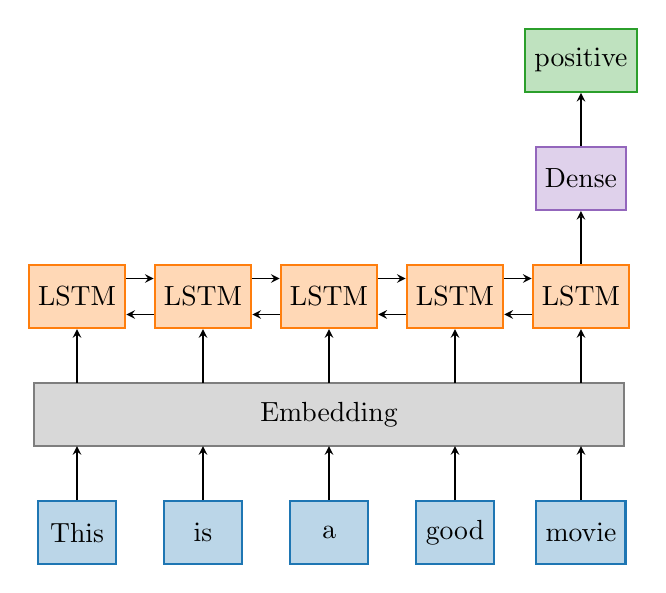
\begin{tikzpicture}
    % boxes
    \foreach \word[count=\x] in {This,is,a,good,movie} {
        \node (in\x) at (1.6*\x, -1.5) [input,token] {\word};
        \node (hidden\x) at (1.6*\x, 1.5) [lstm] {LSTM};
    }
    \node (dense) at (1.6*5, 3) [dense] {Dense};
    \node (out) at (1.6*5, 4.5) [output,token] {positive};
    \node (embedding) at (4.8, 0) [embedding] {Embedding};

    % arrows
    \foreach \x in {1,...,5} {
        \draw [arrow] (in\x.north) to (1.6*\x, -0.4);
        \draw [arrow] (1.6*\x, 0.4) to (hidden\x.south);
    }

    \foreach \x [evaluate=\x as \y using int(\x+1)]  in {1,...,4} {
        \draw [arrow] (hidden\x.20) to (hidden\y.160);
        \draw [arrow] (hidden\y.200) to (hidden\x.340);
    }
    \draw [arrow] (hidden5.north) to (dense.south);
    \draw [arrow] (dense.north) to (out.south);

\end{tikzpicture}
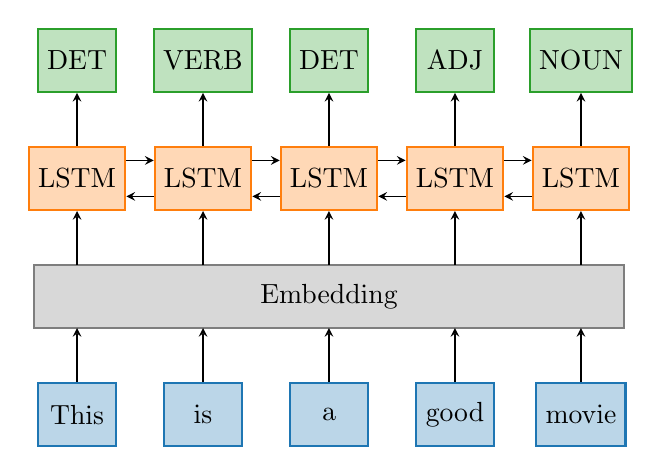
\begin{tikzpicture}
    % boxes
    \foreach \word[count=\x] in {This,is,a,good,movie} {
        \node (in\x) at (1.6*\x, -1.5) [input,token] {\word};
        \node (hidden\x) at (1.6*\x, 1.5) [lstm] {LSTM};
    }
    \node (embedding) at (4.8, 0) [embedding] {Embedding};
    \foreach \tag[count=\x] in {DET,VERB,DET,ADJ,NOUN} {
        \node (out\x) at (1.6*\x, 3) [output,token] {\tag};
    }

    % arrows
    \foreach \x in {1,...,5} {
        \draw [arrow] (in\x.north) to (1.6*\x, -0.4);
        \draw [arrow] (1.6*\x, 0.4) to (hidden\x.south);
        \draw [arrow] (hidden\x.north) to (out\x.south);
    }

    \foreach \x [evaluate=\x as \y using int(\x+1)]  in {1,...,4} {
        \draw [arrow] (hidden\x.20) to (hidden\y.160);
        \draw [arrow] (hidden\y.200) to (hidden\x.340);
    }

\end{tikzpicture}
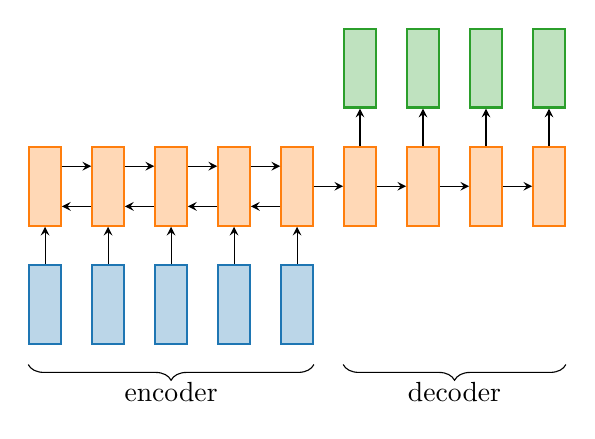
\begin{tikzpicture}
    % boxes
    \foreach \x in {1,...,5} {
        \node (in\x) at (0.8*\x, 0) [input] {};
        \node (hidden\x) at (0.8*\x, 1.5) [hidden] {};
    }
    \foreach \x in {6,...,9} {
        \node (hidden\x) at (0.8*\x, 1.5) [hidden] {};
        \node (out\x) at (0.8*\x, 3) [output] {};
    }

    % arrows
    \foreach \x in {1,...,5} {
        \draw [arrow] (in\x.north) to (hidden\x.south);
    }
    \foreach \x in {6,...,9} {
        \draw [arrow] (hidden\x.north) to (out\x.south);
    }

    \foreach \x [evaluate=\x as \y using int(\x+1)]  in {1,...,4} {
        \draw [arrow] (hidden\x.50) to (hidden\y.130);
        \draw [arrow] (hidden\y.230) to (hidden\x.310);
    }
    \foreach \x [evaluate=\x as \y using int(\x+1)]  in {5,...,8} {
        \draw [arrow] (hidden\x) to (hidden\y);
    }
    \draw[decorate,decoration={brace,amplitude=2mm,raise=0.25cm,mirror}] 
    (in1.south west) -- (in5.south east) 
    node [anchor=north,pos=0.5,yshift=-0.35cm] {encoder}; 

    \gettikzxy{(out6.south west)}{\xstart}{\dummy1}
    \gettikzxy{(in5.south west)}{\dummy2}{\basey}
    \gettikzxy{(out9.south east)}{\xend}{\dummy3}

    \draw[decorate,decoration={brace,amplitude=2mm,raise=0.25cm,mirror}] 
    (\xstart, \basey) -- (\xend, \basey) 
    node [anchor=north,pos=0.5,yshift=-0.35cm] {decoder}; 
    %
    %
    %\draw [
    %    thick,
    %    decoration={
    %        brace,
    %        mirror,
    %        raise=0.5cm
    %    },
    %    decorate
    %] (wall1.east) -- (mass)
    %node [pos=0.5,anchor=north,yshift=-0.55cm] {coil};
\end{tikzpicture}
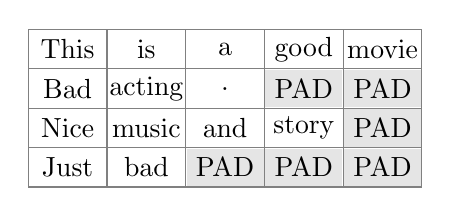
\begin{tikzpicture}
    \draw[xscale=2,step=.5cm,color=gray] (0,0) grid (2.5,2);
    % This is a good movie
    % Terrible acting .
    % Amazing scenery and story
    % Just bad
    \node at (0.5, 1.75) {This};
    \node at (1.5, 1.75) {is};
    \node at (2.5, 1.75) {a};
    \node at (3.5, 1.75) {good};
    \node at (4.5, 1.75) {movie};

    \node at (0.5, 1.25) {Bad};
    \node at (1.5, 1.25) {acting};
    \node at (2.5, 1.25) {.};
    \node at (3.5, 1.25) [pad] {\pad};
    \node at (4.5, 1.25) [pad] {\pad};

    \node at (0.5, 0.75) {Nice};
    \node at (1.5, 0.75) {music};
    \node at (2.5, 0.75) {and};
    \node at (3.5, 0.75) {story};
    \node at (4.5, 0.75) [pad] {\pad};

    \node at (0.5, 0.25) {Just};
    \node at (1.5, 0.25) {bad};
    \node at (2.5, 0.25) [pad] {\pad};
    \node at (3.5, 0.25) [pad] {\pad};
    \node at (4.5, 0.25) [pad] {\pad};

\end{tikzpicture}
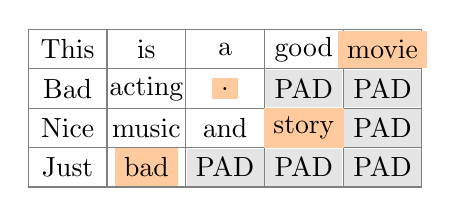
\begin{tikzpicture}
    \draw[xscale=2,step=.5cm,color=gray] (0,0) grid (2.5,2);
    % This is a good movie
    % Terrible acting .
    % Amazing scenery and story
    % Just bad
    \node at (0.5, 1.75) {This};
    \node at (1.5, 1.75) {is};
    \node at (2.5, 1.75) {a};
    \node at (3.5, 1.75) {good};
    \node at (4.5, 1.75) [lastsymbol]{movie};

    \node at (0.5, 1.25) {Bad};
    \node at (1.5, 1.25) {acting};
    \node at (2.5, 1.25) [lastsymbol]{.};
    \node at (3.5, 1.25) [pad] {\pad};
    \node at (4.5, 1.25) [pad] {\pad};

    \node at (0.5, 0.75) {Nice};
    \node at (1.5, 0.75) {music};
    \node at (2.5, 0.75) {and};
    \node at (3.5, 0.75) [lastsymbol]{story};
    \node at (4.5, 0.75) [pad] {\pad};

    \node at (0.5, 0.25) {Just};
    \node at (1.5, 0.25) [lastsymbol]{bad};
    \node at (2.5, 0.25) [pad] {\pad};
    \node at (3.5, 0.25) [pad] {\pad};
    \node at (4.5, 0.25) [pad] {\pad};

\end{tikzpicture}
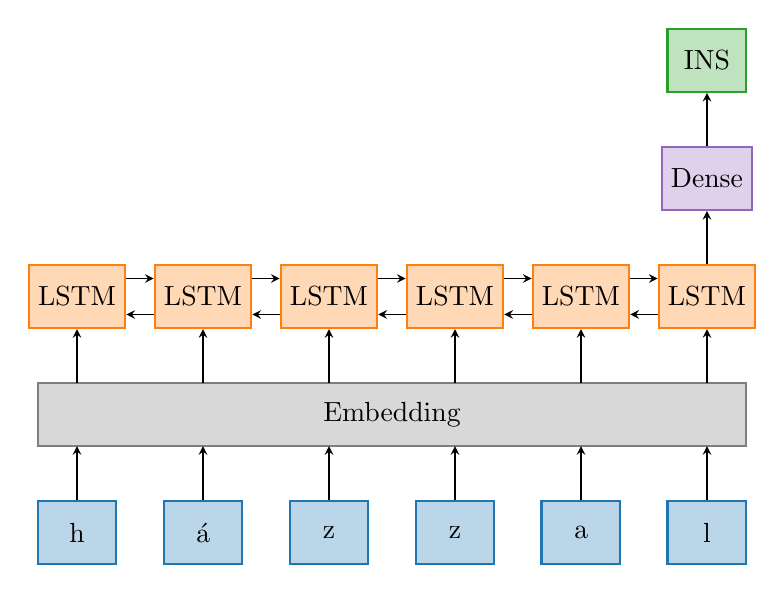
\begin{tikzpicture}
    % boxes
    \foreach \word[count=\x] in {h, á, z, z, a, l} {
        \node (in\x) at (1.6*\x, -1.5) [input,token] {\word};
        \node (hidden\x) at (1.6*\x, 1.5) [lstm] {LSTM};
    }
    \node (dense) at (1.6*6, 3) [dense] {Dense};
    \node (out) at (1.6*6, 4.5) [output,token] {INS};
    \node (embedding) at (5.6, 0) [embedding,minimum width=9cm] {Embedding};

    % arrows
    \foreach \x in {1,...,6} {
        \draw [arrow] (in\x.north) to (1.6*\x, -0.4);
        \draw [arrow] (1.6*\x, 0.4) to (hidden\x.south);
    }

    \foreach \x [evaluate=\x as \y using int(\x+1)]  in {1,...,5} {
        \draw [arrow] (hidden\x.20) to (hidden\y.160);
        \draw [arrow] (hidden\y.200) to (hidden\x.340);
    }
    \draw [arrow] (hidden6.north) to (dense.south);
    \draw [arrow] (dense.north) to (out.south);

\end{tikzpicture}
\end{document}
